\documentclass{sig-alternate}
\usepackage{url}

\title{FriendlyLocation: User Location Estimation Based on the Social Graph}

\numberofauthors{1} 
\author{
    \alignauthor Jeffrey McGee, James Caverlee\\
    \affaddr{Department of Computer Science and Engineering, Texas A\&M
    University} \\
    \affaddr{ College Station, TX 77845 USA} \\
    \email{jeffamcgee@tamu.edu, caverlee@cse.tamu.edu}
} 
\begin{document}

\maketitle
\begin{abstract}
We investigate the relationship between the stregth of the connection between a pair of users, and the distance between the pair.
We use what we have observed about the edges of the social graph to improve a location estimation system.

goal: estimate location of users on twitter
special sauce: people live near friends, some relationships are more important than others, some locations are more precise than others
\end{abstract}




\section{INTRODUCTION}

Publically available data.



\section{RELATED WORK}


\section{DATA COLLECTION}
%\subsection{houston}
%snowball sample starting from a handful of users done in November 2010
%visited @mentioned users and rfriends
%Took everyone who geocoded to Houston, plus users with two out of three:
%    high connectedness using score,
%    central standard time,
%    unknown location field
%Ignored accounts that were protected
%160k users - 80k definite, 80k probable


\subsection{Data from Twitter}
We used Twitter's Streaming API to obtain tweets that contain geographic information.
We used 19877804 tweets posted between April 7 until April 16,2011.
We ignored tweets from users who made their account private, had neither friends nor followers, or posted fewer than two tweets.
We found the median latitude and median longitude for each user, and use this as an approximation of the home location of the user.
We noticed that some Twitter accounts, such as accounts that posted jobs, would move around faster than a human could possibly move. To account for this, we calculated the distance beteen each tweet and the user's home location. We ignored users if the median distance from their tweets to their home location was greater than 50 miles.

We considered users to be in the US based on a simple bounding box.  If their median latitude was between 24 and 50 degrees and their median longitude was between -126 and -66 degrees, then their home location was considered inside the continental US.
We divided these geo-located users into groups based on the last digit of their twitter user id:
\begin{description}
\item[0--6] The training group had 104214 users with a home location in the US bounding box. Some of these users were also used to evaluate the quality of geocoding. For geocoding, we chose users from around the world with a decodable location field and split them into two groups:
\begin{description}
\item[0--3] The geocoding training group has 131295 users.
\item[4--6] The geocoding evalution group has 85664 users.
\end{description}
\item[7--9] The evaluation group had 40861 users with a home location in the US.
\end{description}

For all of the geo-located users who lived in the US, we used Twitter's API to download the users' friends, followers, and 100 most recent tweets.
We also downloaded the profiles for up to 2000 friends, followers, and people they mention in their tweets. If they had over 2000, we chose a random sample of 2000 profiles that included at least 25 of each of the four categories listed below.
From the profiles, we kept the users with a decodable locaion field and threw away the rest. From what was left, we randomly picked one relationship from each of these four categories:
\begin{description}
\item[reciprical friend (rfrd)] The geo-located user follows this user and is followed back.
\item[just friend (jfrd)] The geo-located user follows this user and is not followed back.
\item[just follower (jfol)]The geo-located user is followed by this user, but does not follow them.
\item[just mentioned (jat)] The users do not follow each other, but the geo-located user mentioned the name of the other user in a tweet.
\end{description}
For each of these relationships, we stored their friends, followers, and 100 most recent tweets.

\subsection{Geocoding}
We used Gisgraphy\footnote{\url{http://www.gisgraphy.com/}} to do geocoding.
Gisgraphy does full-text search on the GeoNames\footnote{\url{http://www.geonames.org/}}
database using Lucene. Since
it runs locally we are not limited to a certain number of queries per day.
Gisgraphy's geocoder returns ranked results based on a full text search
over millions of geographical features such as countries, citys, and schools. 

The location field on a user's profile is just a text field that asks the user to respond to "Where in the world are you?".
Repsonses vary from precise latitude and longitude coordinates entered automattically by smart phone apps to jokes and nonsense.
We had to do some preproccessing before sending user-submited locations to the geocoder.
First, we used a regular expression to find latitude and longitude coordinates. These are treated as if they were a unique type of location returned by the geocoder.
Occasionally, users would put two locations seperated by a slash, dash or a conjunction. If the geocoder did not return any results for a user, we tried to geocode both locations and used the first location that the geocoder understood.

We noticed that some locations are significantly more useful than others.
For example, even thogh Rhode Island and Montana are both states with aronud
one million people, Rhode Island is smaller, and as a result, much more useful
in estimating the location of a user.
To make the results of the geocoder more useful, we devised a method to estimate the accuracy of a location returned by the geocoder.
For the users in the geocoding training and evaluation groups, we have both the
home location based on geolocated tweets, and the free-response location field
that we did geocoding on.
Originally, we planned to just use the users in the US, but we found that users
in the US had friends outside of the US, so we need to estimate the quality of
locations outside of the US as well.
As a result, we trained on geographic data from around the world.

We define the location error to be the distance between a user's home location and the result from the geocoder.
The location error can vary from less than a mile to over ten thousand miles.
We ran the geocoder on each user in the geocoding training group, and then grouped users based on the result of the geocoder.
For the 3866 locations that had at least three users, we calculated the median location error for that location.
Next, we grouped all of the locations that had the same type and had one or two users, and calculated the median error for the location type.
We choose the median over average or standard devation because those metrics are strongly affected by large outliers.
We choose to make the cutoff three because that is the smallest value where the median is not just an average.
Table \ref{tab:MedianLocErr} shows the median location error for a few example locations and location types.

We now have a method to predict the quality of a coordinate returned by Gisgraphy.
We define the predicted location error(PLE) for a given location to be median location error if it is one of the 3866 locations that had three users; otherwise, it is the median location error for the location's type.
For example one user had "PDX,OR" in his location field. Gisgraphy identifies this as "Portland International Airport". Since it is not one of the most common locations, its PLE is determined by its place type to be 31 miles as seen in Table \ref{tab:MedianLocErr}.

In Figure \ref{fig:DiffGnpGps}, we show the result of using the PLE to ignore users who have low quality locations such as "Pluto".
The solid black line represents the normal results of geocoding where the location error is less than 1000 miles for 88\% of the users.
The cyan line represents what happens when we remove locations with a PLE greater than or equal to 1000 miles. Now, after removing only 6\% of the users, 93\% of them are within 1000 miles.

\begin{table}
\centering
\caption{Example Median Location Errors}
\begin{tabular}{l r r} 
Location&Number of Users&Median Error in Miles\\ \hline
``Bronx''&53&4\\
``New York''&1264&174\\
``Pluto''\footnote{According to Gisgraphy, Pluto is a city in the Philippines and not a planet.}&11&7843\\ \hline
\\
Place Type&Number of Users&Median Error in Miles\\ \hline
A Coordinate&25216&3\\
A City&7128&6\\
An Airport&117&31\\
A Country&37&3935\\
\hline\end{tabular}
\label{tab:MedianLocErr}
\end{table}

\begin{figure}
\centering
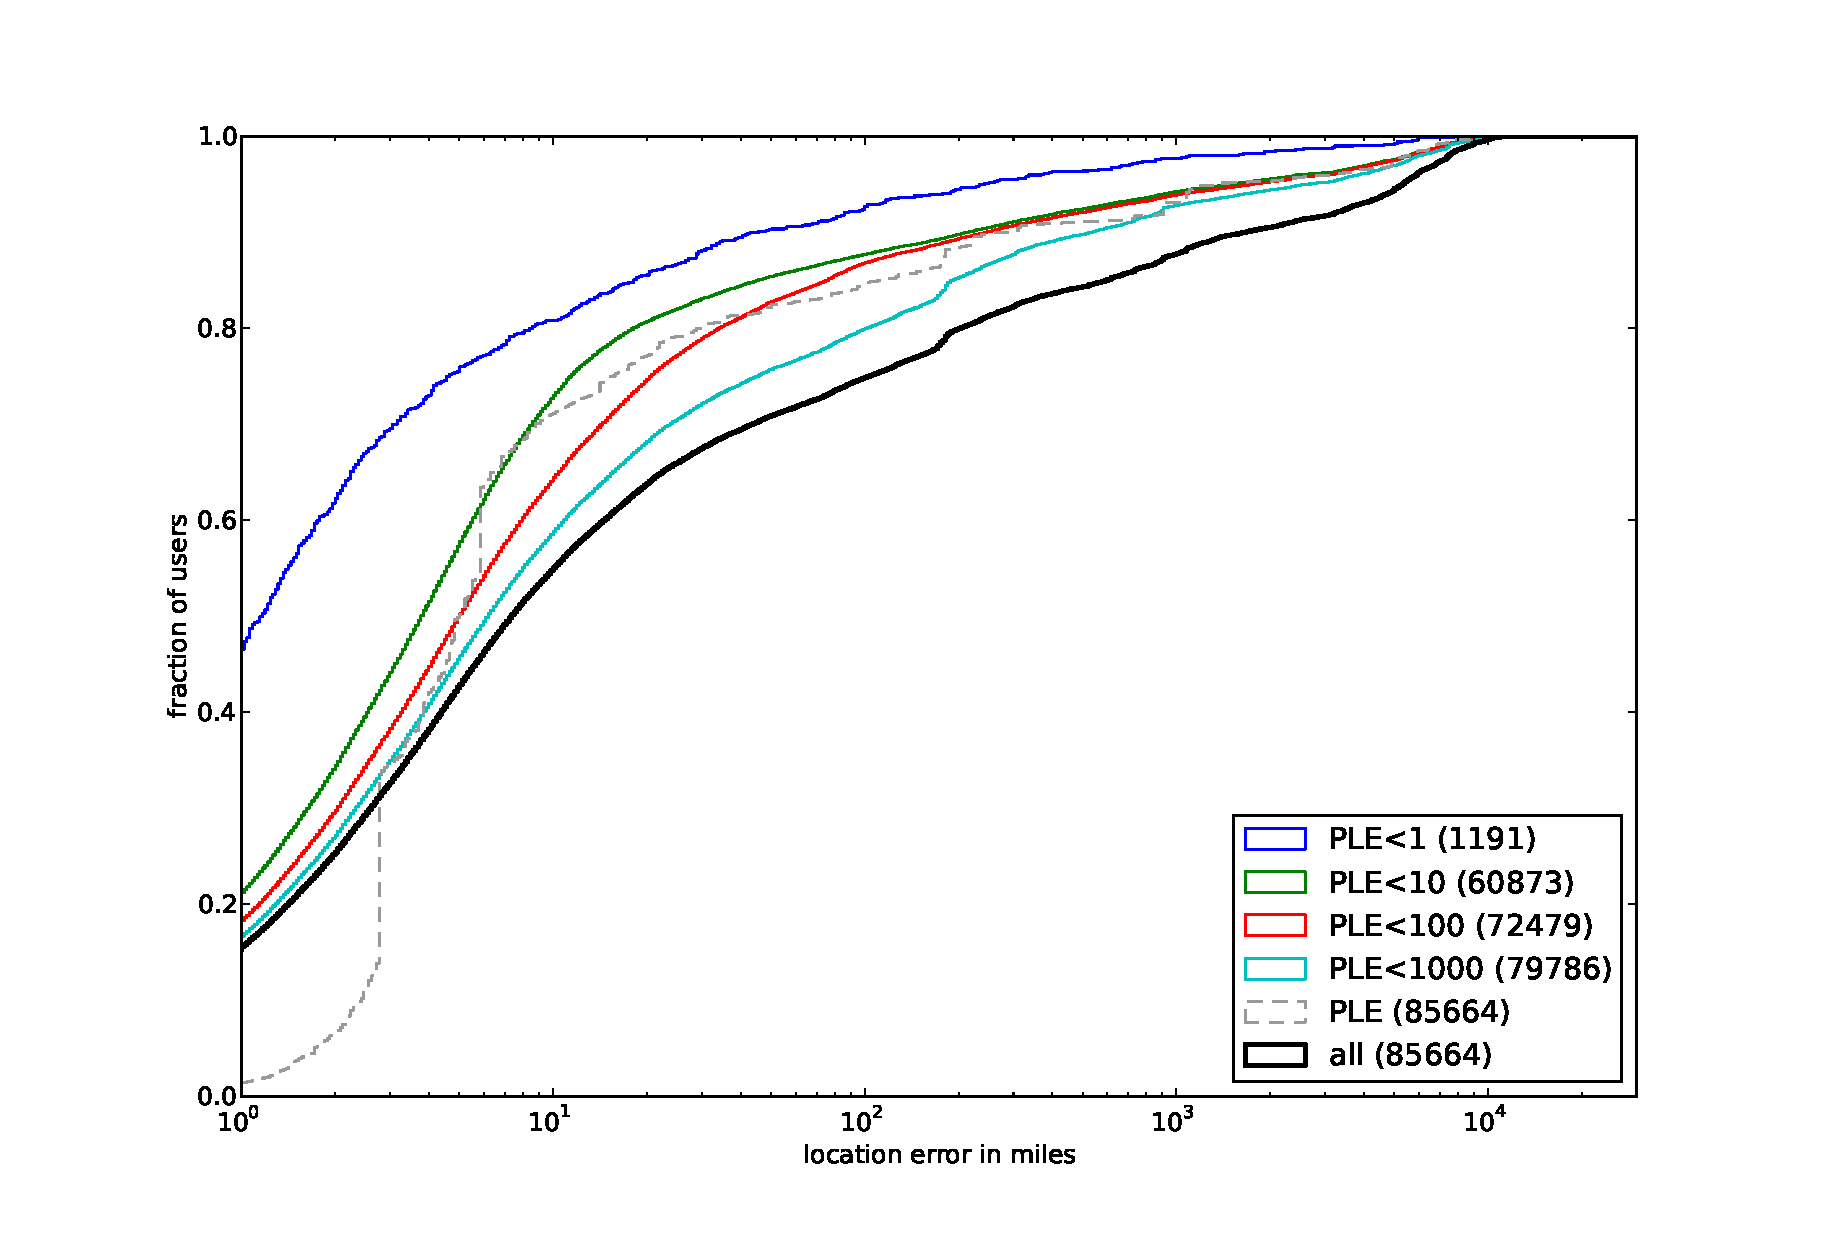
\epsfig{file=diff_gnp_gps.eps, width=\linewidth}
\caption{
The dashed line shows the cumulative distribution of the predicted location error.
The other lines show the  cumulative distribution function of the actual location error for the geocoding evalutation group. The colored lines show how the location prediction improves when we remove users with a high PLE. For example, all the users in the "PLE<1" category have a predicted location error(PLE) of less than one mile.
In the legend, the number in parenthesis is the number of users in that category.
}
\label{fig:DiffGnpGps}
\end{figure}

\section{INVESTIGATION}

All of the analysis in this section of this document was done on 104214 users with a home location inside the US bounding box


What type of friendship is closest?

What is the relationship between friendship and distance?
mixed social network and news network
some connections are based on 

Are you closer to people you commmunicate with?















analysis of Houston:
most users stay within 8 miles of home
users tweet along roadways
geolocoated tweets show map starting at houston expanding out
looked at triangles posting distance of two sides on x-y axis
strong concentration at 0,0
compared fake triangles to real triangles:
    real triangles have high concentration near origin
    fake triangles spread out
%hou_gis: where locations tend to resolve to
Since people often say they live in a city, there are large clusters.

For houston, I picked a friend for each user and went from there.
In houston data, having stars in common hurts the chances that two users are nearby.  It doesn't matter for the geo data. In Houston, we are only looking at up to 100 miles. Does this matter?


%normed_edges.png:
conv>ated>at>rfrd>fol>frd>random
why is rfrd so close to fol in the hou data? Because we know they live near eachother?

%tpu_hist: tweets per user is zipfian

%diff_gnp_gps.png - shows the error in gnp decoding by comparing it to normal tweets

%tri_deg_*.png - The number of triangles formed is NOT a function of the number of edges a user has therefore talking about the ratio of people involved in a type of triangle is stupid.

%geo_edges_log.png - same as normed_edges.png

%geo_tri_rfrd_sp.png - distance is a binomial distribution, possibly the sum of two log-normal distributions.

%geo_local_1_*.png when you take out non-locals the cumulative graph starts to look linear.

%geo_local_*.png - after removing the non-local, you still see a hump around 10 miles. Is that just error from the geo-coding and city level data?

%local_ratio.png - star v. non-star matters a lot for friend case, but not so much in others
\section{EVALUATION}
\section{FUTURE WORK}

\bibliographystyle{abbrv}
\bibliography{fl} 
\end{document}
